\documentclass[11pt,a4paper]{article}
\usepackage[T1]{fontenc}
\usepackage[utf8]{inputenc}
\usepackage{lmodern}
\usepackage{amsmath,amssymb,amsthm,mathtools,mathrsfs}
\usepackage{graphicx,float,xcolor,multicol}
\usepackage[shortlabels]{enumitem}
\usepackage[margin=27mm]{geometry}
\usepackage{microtype,needspace,placeins}
\usepackage{tikz,tikz-cd}
\usetikzlibrary{arrows.meta,calc,positioning,patterns,decorations.pathreplacing}
\usepackage[colorlinks=true,linkcolor=teal,urlcolor=teal,citecolor=teal]{hyperref}
\setlength{\parindent}{0pt}
\setlength{\parskip}{.6em}
\setcounter{secnumdepth}{0}
\allowdisplaybreaks
\raggedbottom
\providecommand{\cross}{\times}
\DeclareUnicodeCharacter{2020}{\ensuremath{\dagger}}
\DeclareMathOperator{\supp}{supp}
\DeclareMathOperator*{\esssup}{ess\,sup}
\providecommand{\chapter}{\section}
\newenvironment{tool}[2]{\subsection*{Tool #1 --- #2}}{}
\newcommand{\ToolRef}[1]{Tool #1}
\newcommand{\FigureTag}[2]{\textit{Figure #1}}
\newcommand{\Result}[1]{\subsection*{#1}}
\newcommand{\Application}[1]{\subsubsection*{Application\if\relax\detokenize{#1}\relax\else\space--- #1\fi}}
\newcommand{\ProofHeading}{\par\textit{Proof.}\space}
\newcommand{\ProofOf}[1]{\par\textit{Proof of #1.}\space}
\newcommand{\RemarkHeading}{\par\textbf{Remark.}\space}
\newcommand{\NoteHeading}{\par\textbf{Note.}\space}
\newcommand{\ExerciseHeading}{\par\textbf{Exercise.}\space}

% Rendering support only; mathematical text is in each independent post.
\usepackage{booktabs,array,longtable}
\definecolor{HandoutBlue}{HTML}{2F6690}
\definecolor{HandoutNavy}{HTML}{17365D}
\newtheorem{theorem}{Theorem}
\newtheorem{lemma}[theorem]{Lemma}
\newtheorem{proposition}[theorem]{Proposition}
\newtheorem{corollary}[theorem]{Corollary}
\newtheorem{conjecture}[theorem]{Conjecture}
\newtheorem{definition}{Definition}
\newtheorem{example}{Example}
\newtheorem{namedtoolcounter}{Tool}
\newenvironment{namedtool}[1]{\begin{namedtoolcounter}[#1]}{\end{namedtoolcounter}}
\newtheorem*{claim}{Claim}
\newtheorem*{remark}{Remark}
\newtheorem*{exercise}{Exercise}
\newtheorem*{question}{Question}
\newtheorem*{observation}{Observation}
\newcommand{\SourceChapter}[2]{\section*{#2}}
\newcommand{\Lecture}[2]{\section*{Lecture #1: #2}}
\newcommand{\unclear}[1]{\textit{[unclear: #1]}}
\newcommand{\sourcegap}{\textit{[unfinished in the source]}}
\DeclareMathOperator{\dist}{dist}
\DeclareMathOperator{\id}{id}
\DeclareMathOperator{\Hol}{Hol}
\DeclareMathOperator{\Per}{Per}
\DeclareMathOperator{\Fix}{Fix}
\DeclareMathOperator{\diam}{diam}
\DeclareMathOperator{\Var}{Var}
\DeclareMathOperator{\Leb}{Leb}
\DeclareMathOperator{\Hom}{Hom}
\DeclareMathOperator{\End}{End}
\DeclareMathOperator{\Ann}{Ann}
\DeclareMathOperator{\Spec}{Spec}
\DeclareMathOperator{\Max}{Max}
\DeclareMathOperator{\Ob}{Ob}
\DeclareMathOperator{\Tor}{Tor}
\DeclareMathOperator{\Ass}{Ass}
\DeclareMathOperator{\Mor}{Mor}
\DeclareMathOperator{\Fun}{Fun}
\DeclareMathOperator{\Nat}{Nat}
\DeclareMathOperator{\Cone}{Cone}
\DeclareMathOperator{\MCG}{MCG}
\DeclareMathOperator{\Aut}{Aut}
\DeclareMathOperator{\Deck}{Deck}
\DeclareMathOperator{\SL}{SL}
\DeclareMathOperator{\PSL}{PSL}
\DeclareMathOperator{\Area}{Area}
\DeclareMathOperator{\im}{im}
\DeclareMathOperator{\PSh}{PSh}
\newcommand{\CRing}{\mathsf{CRings}}
\newcommand{\AMod}{A\text{-}\mathsf{Mod}}
\newcommand{\Ab}{\mathsf{Ab}}
\newcommand{\Z}{\mathbb Z}
\newcommand{\Q}{\mathbb Q}
\newcommand{\R}{\mathbb R}
\newcommand{\C}{\mathbb C}
\newcommand{\N}{\mathbb N}
\newcommand{\kk}{\mathbb k}
\renewcommand{\aa}{\mathfrak a}
\newcommand{\bb}{\mathfrak b}
\newcommand{\pp}{\mathfrak p}
\newcommand{\qq}{\mathfrak q}
\newcommand{\mm}{\mathfrak m}
\newcommand{\nn}{\mathfrak n}
\newcommand{\rad}{\mathrm r}
\newcommand{\cat}[1]{\mathsf{#1}}
\setcounter{secnumdepth}{0}
\allowdisplaybreaks

\graphicspath{{figures/ergodic-theory/}}
\begin{document}
\section*{Equidistribution}
% BLOG-CONTENT-BEGIN

\begin{remark}[1]
Notice that Choquet's theorem implies that $\lvert\mathcal M^T(X)\rvert=1$
if $\lvert\mathcal E^T(X)\rvert=1$, for $\mathcal M^T(X)$ consists of
``convex linear combinations'' of elements of $\mathcal E^T(X)$.
\end{remark}


\setcounter{definition}{9}\begin{definition}[Equidistribution]
We say that $(x_n)_n$, with $x_n\in X$, is \emph{equidistributed} in $(X,T)$
if, for every $f\in C(X)$, we have
\[
  \lim_{n\to\infty}\frac1n\sum_{j=1}^n f(x_j)
  =\int_X f(x)\,d\mu(x).
\]
\end{definition}



% Source page 5
To see what equidistribution means probabilistically, one must go to $[0,1]$.
There we have the following.

\setcounter{theorem}{24}\begin{lemma}
Let $[0,1]$, equipped with Lebesgue measure, be our setting. If $(x_n)_{n\geq1}$
is equidistributed, then
\[
  \lim_{n\to\infty}\frac1n
  \bigl|\{j:1\leq j\leq n,\ x_j\in[a,b]\}\bigr|=b-a.
\]
\end{lemma}

In other words, equidistribution means being uniformly distributed over
$[0,1]$. We have the same for ergodic orbits in the more general setting of
a probability measure space, but those are special sequences regardless of
how general the setting is: notice that $\mathcal E^T(X)$ is merely the set
of extremal points of $\mathcal M^T(X)$.

\Needspace{7cm}
\begin{proof}
\begin{figure}[H]
  \centering
  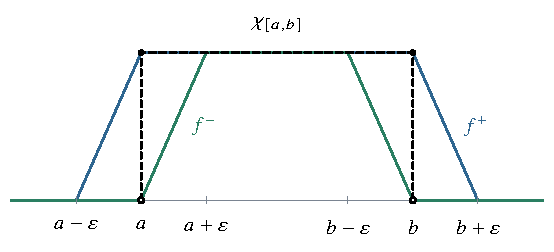
\includegraphics[width=.62\textwidth]{lecture7-fig-01.pdf}
  \FigureTag{L7.1}{fig:lecture7-fig-01}
\end{figure}
Let $f^-$ and $f^+$ be as shown in the figure. Note that
$f^-\leq\chi_{[a,b]}\leq f^+$, and one can arrange $f^\pm$ so that
\[
  \int_0^1(f^+-f^-)(x)\,dx\leq2\varepsilon.
\]

% Source page 6
\begin{align*}
  b-a-2\varepsilon
  &\leq\int_0^1f^-\,dx
  \leq\liminf_{N\to\infty}A_N^{\chi_{[a,b]}}
  \leq\limsup_{N\to\infty}A_N^{\chi_{[a,b]}}\\
  &\leq\int_0^1f^+\,dx\leq b-a+2\varepsilon.
\end{align*}
Thus $\liminf_{N\to\infty}A_N^{\chi_{[a,b]}}
=\limsup_{N\to\infty}A_N^{\chi_{[a,b]}}=b-a$.
\end{proof}


We have dealt with one of the problems raised in Lecture 5, that of ergodic
decomposition. In the next few lectures, let us deal with the problem of
classifying systems up to measurable isomorphisms.
% BLOG-CONTENT-END
\end{document}
